\section{Fallstudie}
In diesem Kapitel wird die technische Realisierung einer Fallstudie beschrieben. Dabei werden sowohl die verwendeten Technologien als auch die eintretenden beziehungsweise zu verarbeitenden Szenarien sowie deren Implementierung erläutert.

\subsection{Verwendete Technologien}
Damit die Fallstudie in einer angemessenen Art präsentiert werden kann, erfolgt die Realisierung des Projekts als Web-Applikation. Dafür wird mit \textit{Spring-Boot} ein quell-offenes Java-Framework verwendet. Darin enthaltene Komponenten wie \textit{SpringMVC} und der Applikation-Server \textit{Tomcat} ermöglichen eine konfigurationsarme Erstellung der Webanwendung. Die Webanwendung besteht im Wesentlichen aus einer serverseitigen (Backend) und einer clientseitigen (Frontend) Komponente.\\
Das Backend folgt dem Architekturmuster \textit{Model-View-Controller}. Die Controller-Klassen stellen REST-Schnittstellen bereit, durch die es möglich ist, einzelne Events zu senden und diese durch eine \textit{Complex Event Processing} - Engine (CEP) zu verarbeiten.\\
Das Frontend wird durch Verwendung der \textit{Java Server Pages} - Technologie (JSP) in Kombination mit der \textit{Java Standard Tag Library} (JSTL) umgesetzt. Diese ermöglicht die Visualisierung des aktuellen Zustands des Straßenausschnitts, die Steuerung von Eventströmen und die Steuerung der Events. Die Kommunikation zwischen Front- und Backend erfolgt durch den Einsatz von AJAX (\textit{Asynchrounous JavaScript and XML}).\\
Als CEP - Engine wird \textit{Esper} verwendet. Esper ermöglicht die schnelle Verarbeitung großer Mengen eingehender Nachrichten und ist somit sehr gut für die Verwendung in Smart Traffic Szenarien geeignet. 


\subsection{Beschreibung der Ausgangslage}
Das Szenario dieser Fallstudie beschreibt den fiktiven Kartenausschnitt aus Abb.\ref{fig2}. Dieser Ausschnitt besteht aus den drei Kreuzungen K1, K2 und K3, einer Nord-Süd-Achse S3 und einer West-Ost-Achse S1 als Hauptverkehrsstraßen sowie einen Bahnübergang welcher die West-Ost-Achse kreuzt. Die Verkehrsteilnehmer sind autonom fahrende (Einsatz-)Fahrzeuge, deren Fahrtrichtung durch Pfeile in den Tabellen auf Abb.\ref{fig2} dargestellt werden. Die für die Fahrzeuge relevante Tabelle befindet sich jeweils an der rechten Seite in Fahrtrichtung. Die grün umrandete Tabelle gibt als Beispiel die Fahrtrichtung für die aus westlicher Richtung auf der Straße S1 fahrenden Fahrzeuge vor. Die Ereignisse in dieser Fallstudie beschränken sich auf die Kreuzung K2. Aus diesem Grund erfolgt die Verkehrslenkung an den Kreuzungen K1 und K3, weshalb für K2 keine Tabellen dargestellt werden. Als Ausweichrouten können die parallel verlaufende nördliche Straße S2 sowie die westlich von der S3 verlaufende S4 befahren werden. Diese werden verwendet, wenn es die Verkehrslage durch eines oder mehrere der möglichen nachfolgend aufgelisteten Szenarien erfordert.

\begin{itemize} 
\item Unfall an Kreuzung K2
\item Geschlossene Bahnschranke
\item Erhöhte Stickstoffbelastung an Kreuzung K2
\item Überhöhtes Verkehrsaufkommen an Straße S1
\end{itemize}

\begin{figure}[ht]
	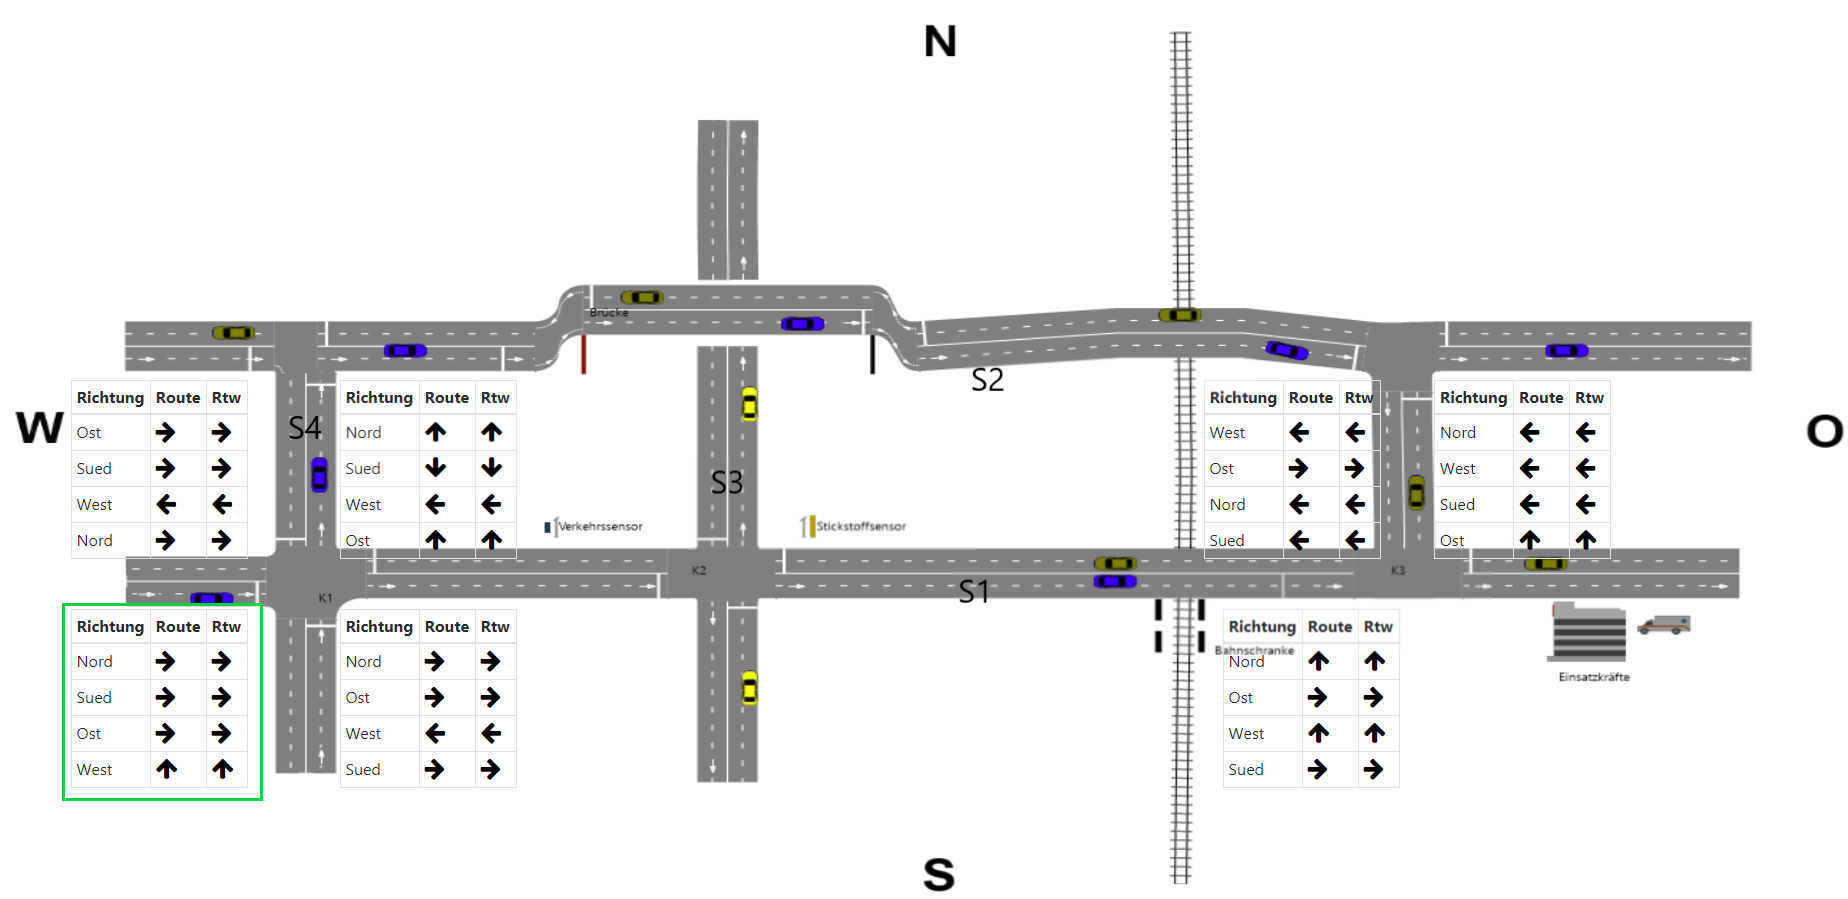
\includegraphics[width=\textwidth]{images/dataanalyticswebapp.png}
	\caption{Straßenausschnitt mit Anzeige der Fahrrichtung}
	\label{fig2}
\end{figure}

Nachdem die Ausgangslage der Fallstudie beschrieben wurde, werden die oben genannten Events in den nachfolgenden Abschnitten genauer beschrieben. Dabei werden sowohl die eingesetzten Statements als auch die Auswirkung der eintretenden Ereignisse auf das vorgestellte Szenario erläutert. Jedes Event enthält ein Attribut welches den Ort des Ereignisses beinhaltet. Durch diesen können mehrere gleichartige Ereignisse an unterschiedlichen Orten überwacht werden. Die Fahrtrichtungspfeile, die sich durch ein eingetretenes Ereignis ändern, werden grün hervorgehoben.

\subsection{Steuerung der Ereignisse}
Die Steuerung der Ereignisse erfolgt wie bereits erwähnt über die WebUI. Dabei wird zwischen dem Verkehrsstrom als kontinuierlich auftretende Ereignisse und Einzelereignissen \textit{Bahnschranke}, \textit{Verkehrslage K2} und \textit{Stickoxid-Werte K2} unterschieden. Die Felder in Abb. \ref{fig5} dienen der Auslösung der Einzelereignisse.

\begin{figure}[ht]
\begin{center}
	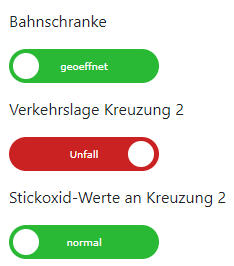
\includegraphics[scale=0.7]{images/EventTrigger.png}
	\caption{Auslöser für Events}
	\label{fig5}
\end{center}
\end{figure}

Die Regelung des Verkehrsstroms erfolgt über die in Abb. \ref{fig12} beispielhaft dargestellten Eingabefelder. Diese Intervallwerte repräsentieren einen Verkehrssensor, welcher die angegebene Anzahl an Autos detektiert. Über separate Threads werden im Backend die Anzahl der Autos in \textit{TrafficStartEvents} übersetzt und kontinuierlich in den Ereignisstrom übergeben. Diese Events beinhalten ein Attribut zur Angabe der gewünschten Fahrtrichtung, um sie für Esper unterscheidbar zu machen.

\begin{figure}[ht]
\begin{center}
	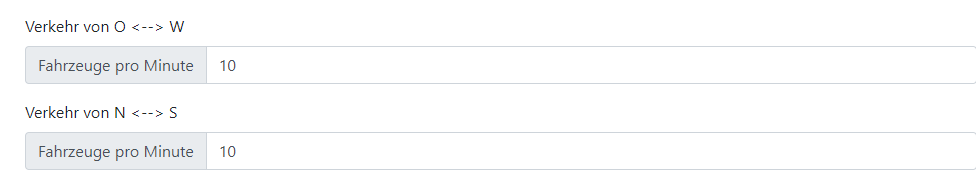
\includegraphics[width=\textwidth]{images/verkehrsstrom.png}
	\caption{Fahrzeuge pro Minute je Fahrtrichtung}
	\label{fig12}
\end{center}
\end{figure}

Die Verarbeitung der Ereignismuster durch Esper wird in den nachfolgenden Abschnitten erläutert.
\subsection{Unfall an Kreuzung} \label{accident}

Sobald das Feld \textit{Verkehrslage Kreuzung 2} ausgelöst wird, wird ein \textit{AccidentStartEvent} in den Ereignisstrom gesendet. Durch das Statement 

\begin{lstlisting}
select crossing from AccidentStartEvent
\end{lstlisting}

erkennt Esper das Event und löst einen \textit{AccidentStartListener} aus. Abb. \ref{fig6} zeigt die Änderungen der Fahrtrichtungen, die im \textit{AccidentStartListener} ausgelöst werden.  
Dieser ändert die Fahrtrichtungen dahingehend, dass Einsatzfahrzeuge weiterhin die Straße S1 befahren dürfen und der restliche Verkehr über die Nordumgehung S2 umgeleitet wird. 

\begin{figure}[ht]
	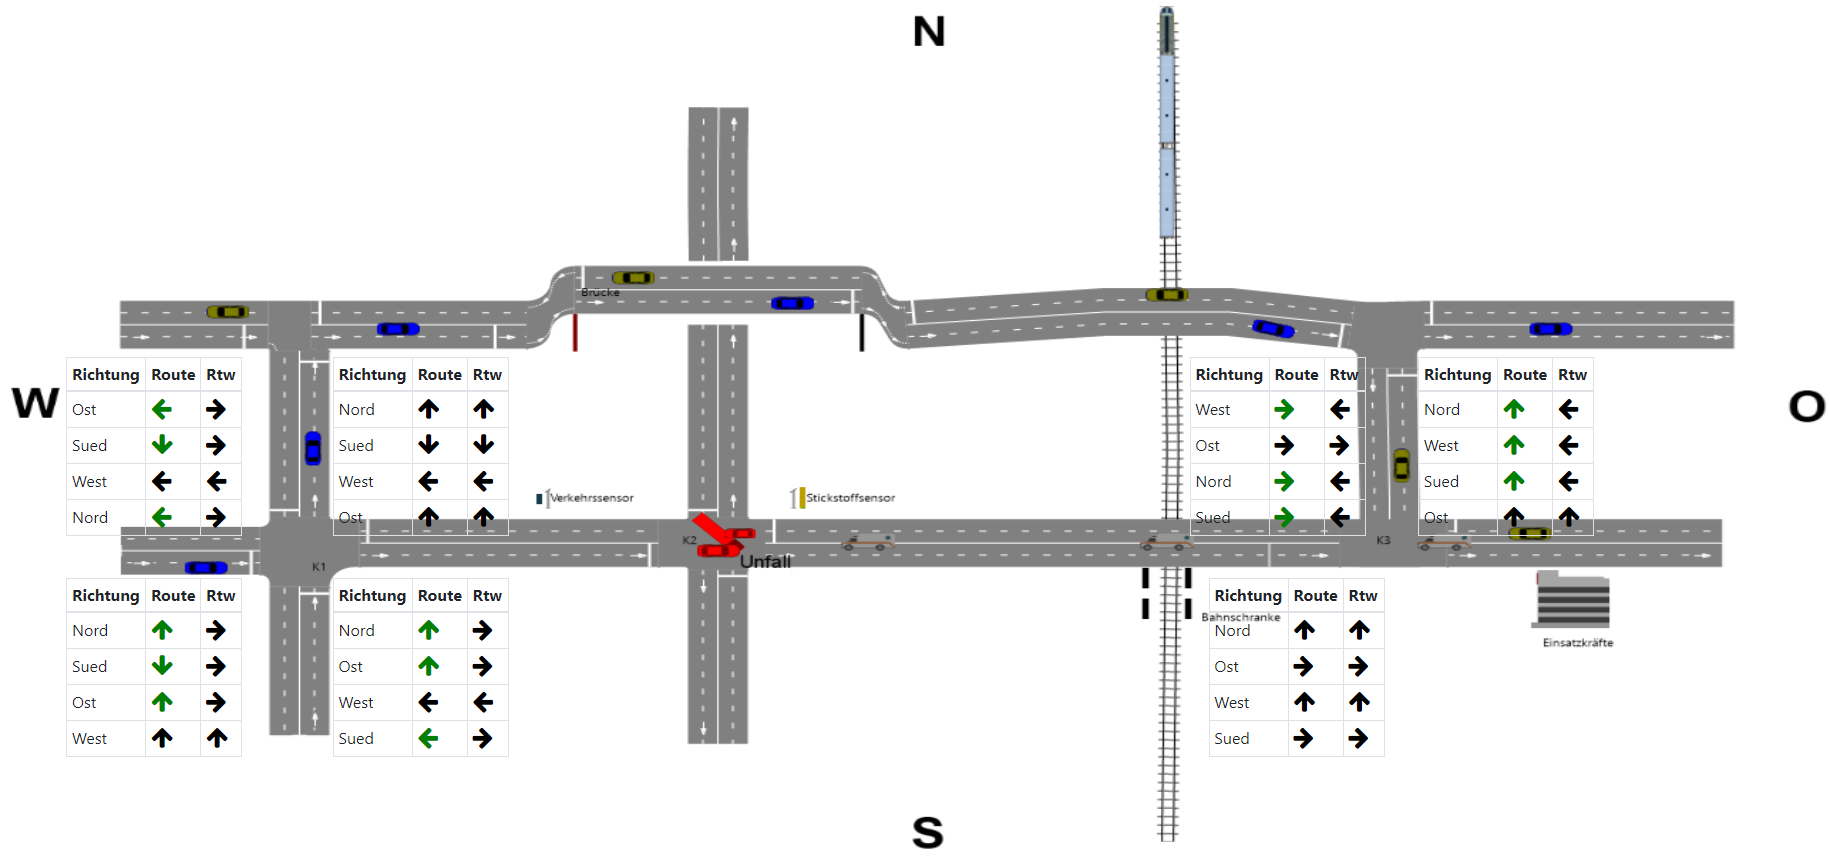
\includegraphics[width=\textwidth]{images/Accident.png}
	\caption{Unfall an K2 und Umleitung der Fahrzeuge außer Einsatzfahrzeuge}
	\label{fig6}
\end{figure}

Damit im Anschluss an den Unfall die Verkehrsführung angepasst werden kann, werden zwei weitere Statements verwendet. Dabei muss die aktuelle Situation am Bahnübergang beachtet werden. Das nachfolgende Statement prüft, ob zusätzlich zum \textit{AccidentEndEvent} die \textit{RailroadCrossingBarrierClose-} und \textit{RailroadCrossingBarrierOpenEvents} in der gleichen Häufigkeit ausgelöst wurden. Somit kann unterschieden werden, ob die Schranke zu dem Zeitpunkt geöffnet (gleiche Häufigkeit) oder geschlossen ist. 

\begin{lstlisting}
select crossing from AccidentEndEvent where ( (select count(*) from RailroadCrossingBarrierCloseEvent) = (select count(*) from RailroadCrossingBarrierOpenEvent))
\end{lstlisting}

Ist dies der Fall, reagiert der \textit{AccidentEndBarrierOpenListener}. Dieser setzt die Verkehrsführung auf die Ausgangslage wie in Abb. \ref{fig5} zurück. Zur Abdeckung der Möglichkeit, dass nach Unfallende die Bahnschranke geschlossen ist, kommt das Statement

\begin{lstlisting}
select crossing from AccidentEndEvent where ( (select count(*) from RailroadCrossingBarrierCloseEvent) != (select count(*) from RailroadCrossingBarrierOpenEvent))
\end{lstlisting}

zum Einsatz. Dieses wird ausgelöst wenn die Anzahl an \textit{RailroadCrossingBarrierCloseEvent} und \textit{RailroadCrossingBarrierOpenEvents} nicht den gleichen Wert ausweisen. Dann wird der \textit{AccidentEndBarrierClosedListener} ausgeführt und die Verkehrslage entspricht der im nachfolgenden Abschnitt erläuterten Situation.

\subsection{Geschlossene Bahnschranke} \label{closedBarrier}

Diese Situation wird nach der Aktivierung der Schaltfläche \textit{Bahnschranke} durch den Eingang eines \textit{RailroadCrossingBarrierCloseEvent} im Ereignisstrom  erkannt. Das dafür verwendete Statement

\begin{lstlisting}
select railwayCrossing from RailroadCrossingBarrierCloseEvent
\end{lstlisting}

löst den \textit{BarrierCloseListener} aus, welcher die in Abb. \ref{fig7} dargestellte Reaktion umsetzt.

\begin{figure}[ht]
	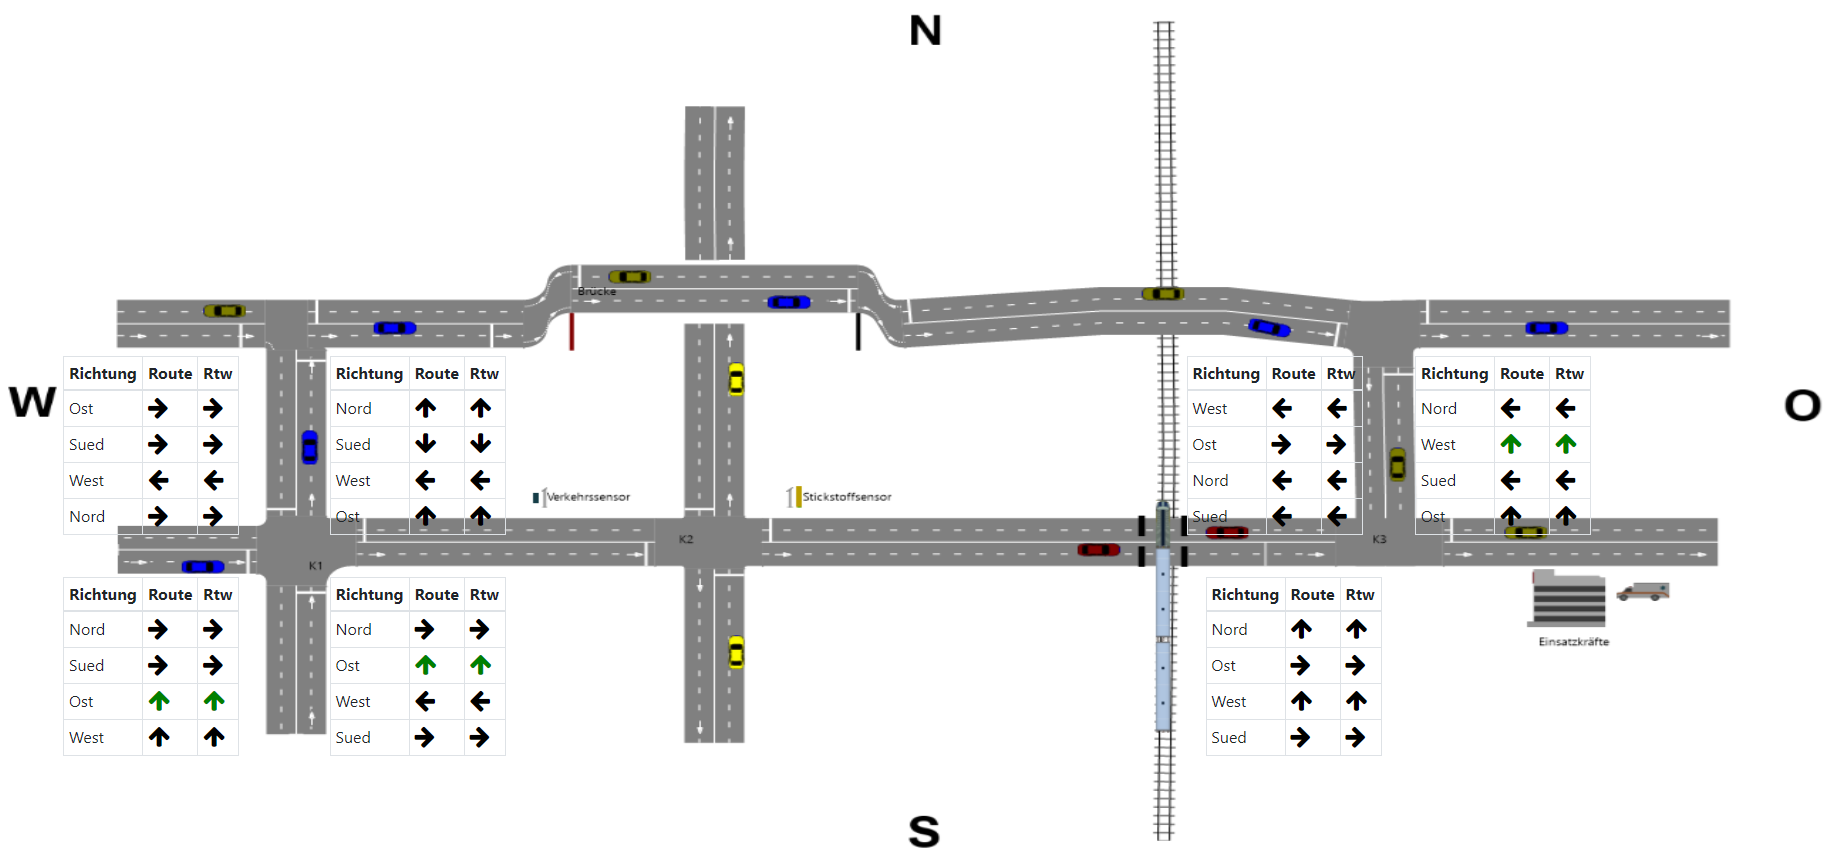
\includegraphics[width=\textwidth]{images/RailroadBarrierClose.png}
	\caption{Geschlossene Bahnschranke und Umleitung der Fahrzeuge aus Ost, West und Südwest}
	\label{fig7}
\end{figure}

Ähnlich wie beim Unfallereignis muss nach Beendigung durch ein \textit{RailroadCrossingBarrierCloseEvent} überprüft werden, ob an der Kreuzung K2 ein Unfallereignis aktiv ist. Dies geschieht durch die zwei Statements 

\begin{lstlisting}
select railwayCrossing from RailroadCrossingBarrierOpenEvent where ( (select count(*) from AccidentStartEvent) = (select count(*) from AccidentEndEvent))
\end{lstlisting}

\begin{lstlisting}
select railwayCrossing from RailroadCrossingBarrierOpenEvent where ( (select count(*) from AccidentStartEvent) != (select count(*) from AccidentEndEvent))
\end{lstlisting}

die nach dem gleichen Prinzip wie in Absatz \ref{accident} prüfen, ob die Anzahl an \textit{AccidentStart-} und \textit{AccidentEndEvents} gleich ist.\\
Ist ein Unfallereignis aktiv, werden die Fahrzeuge gemäß dem Unfallereignis umgeleitet. Andernfalls werden die Fahrzeuge wieder über die optimalen Routen geführt.


\subsection{Erhöhte Stickstoffbelastung}

Ein Stickstoffalarm wird durch die Aktivierung der Schaltfläche \textit{Stickoxid-Werte an Kreuzung 2} und dem aktionsverbunden Versand eines \textit{NitrogenOxideStartEvent} an den Ereignisstrom ausgelöst. Das Statement

\begin{lstlisting}
select crossing from NitrogenOxideStartEvent
\end{lstlisting}

erfasst das Ereignis und löst den \textit{NitroOxigenHighListener} aus. In Abb. \ref{fig8} ist ersichtlich wie daraufhin in einer ersten Eskalationsstufe zur Reduzierung der Schadstoffbelastung, der Ost-West-Verkehr über die Umgehungsstraße geleitet wird. 

\begin{figure}[ht]
	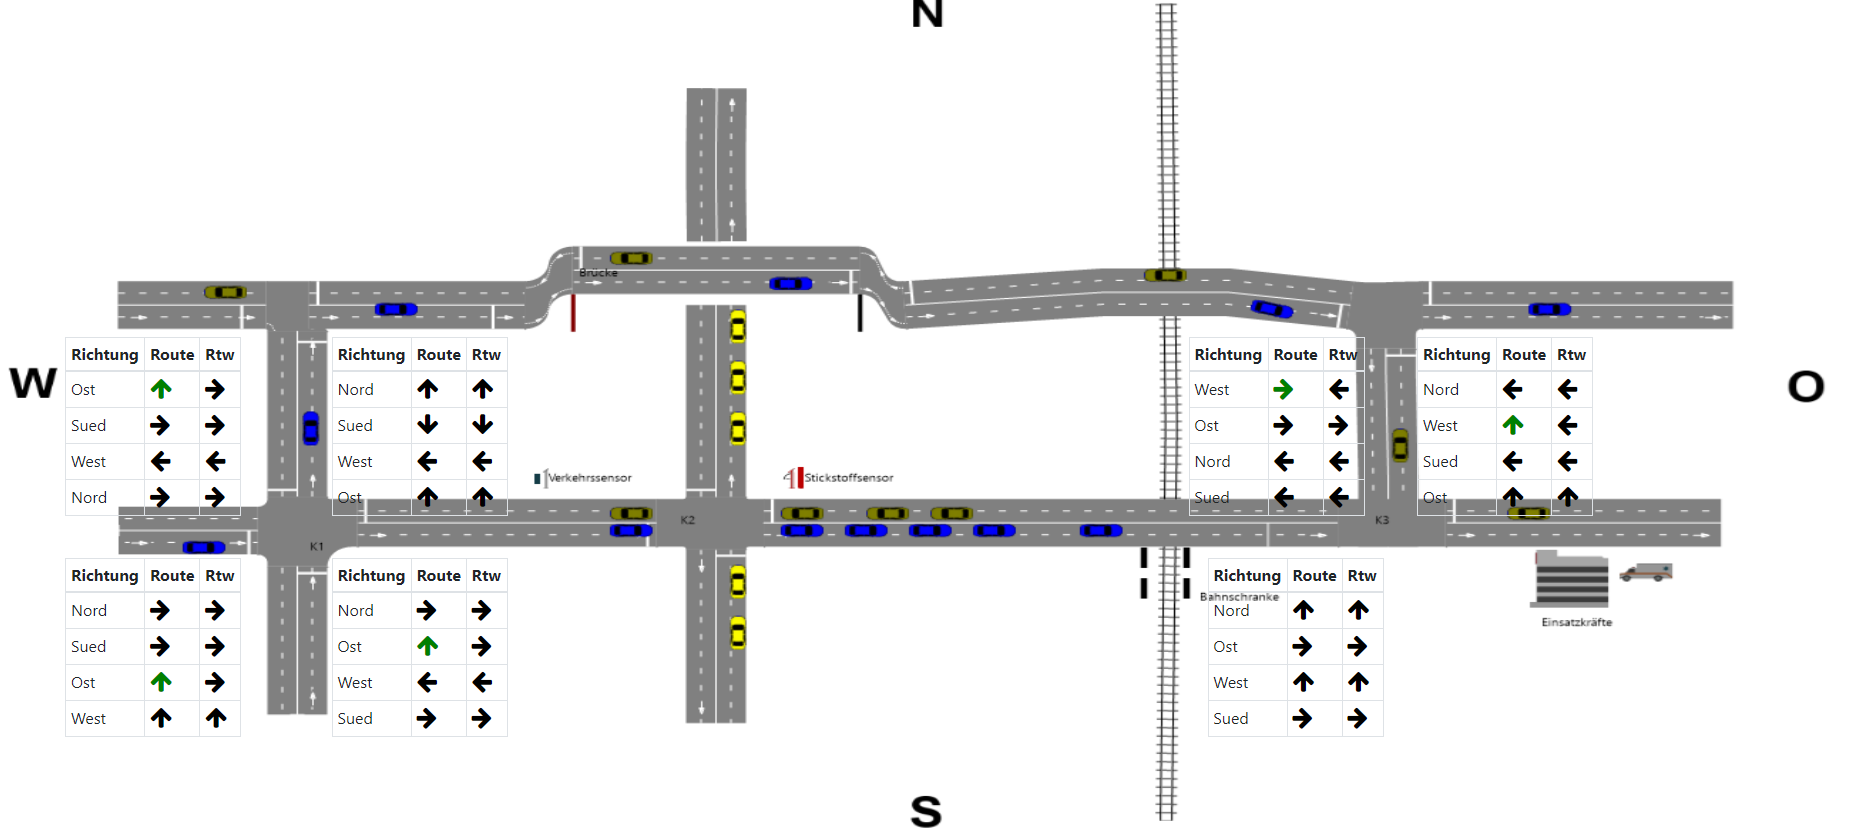
\includegraphics[width=\textwidth]{images/NitroOxigenHigh.png}
	\caption{Stickstoff-Warnung und Sperrung für Ost-West-Verkehr}
	\label{fig8}
\end{figure}

Parallel dazu wird durch das Statement

\begin{lstlisting}
select a,b from pattern [every a = NitrogenOxideStartEvent(crossing = 'k2') -> (timer:interval(10 seconds) and b = NitrogenOxideEndEvent(crossing = a.crossing))]
\end{lstlisting}

geprüft, ob nach Auftreten des \textit{NitrogenOxideStartEvent} an Kreuzung K2 innerhalb eines definierten Zeitintervalls ein \textit{NitroOxideEndEvent} an der gleichen Kreuzung erfasst wurde. Ist das der Fall, wird die Straße S1 für den Ost-West-Verkehr wieder freigegeben. Im Gegenzug prüft das Statement

\begin{lstlisting}
select a,b from pattern [every a = NitrogenOxideStartEvent(crossing = 'k2') -> (timer:interval(10 seconds) and not b = NitrogenOxideEndEvent(crossing = a.crossing))]
\end{lstlisting}

ob in dem definierten Zeitraum an der Kreuzung kein \textit{NitrogenEndEvent} erfasst wurde. Dann wird der \textit{NitroOxigenTimeIntervalListener} ausgelöst und stößt die nächste Eskalationsstufe an. Diese ist in Abb. \ref{fig9} dargestellt und zeigt die zusätzliche Sperrung für Zufahrten auf die Nord-Süd-Verbindung.

\begin{figure}[ht]
	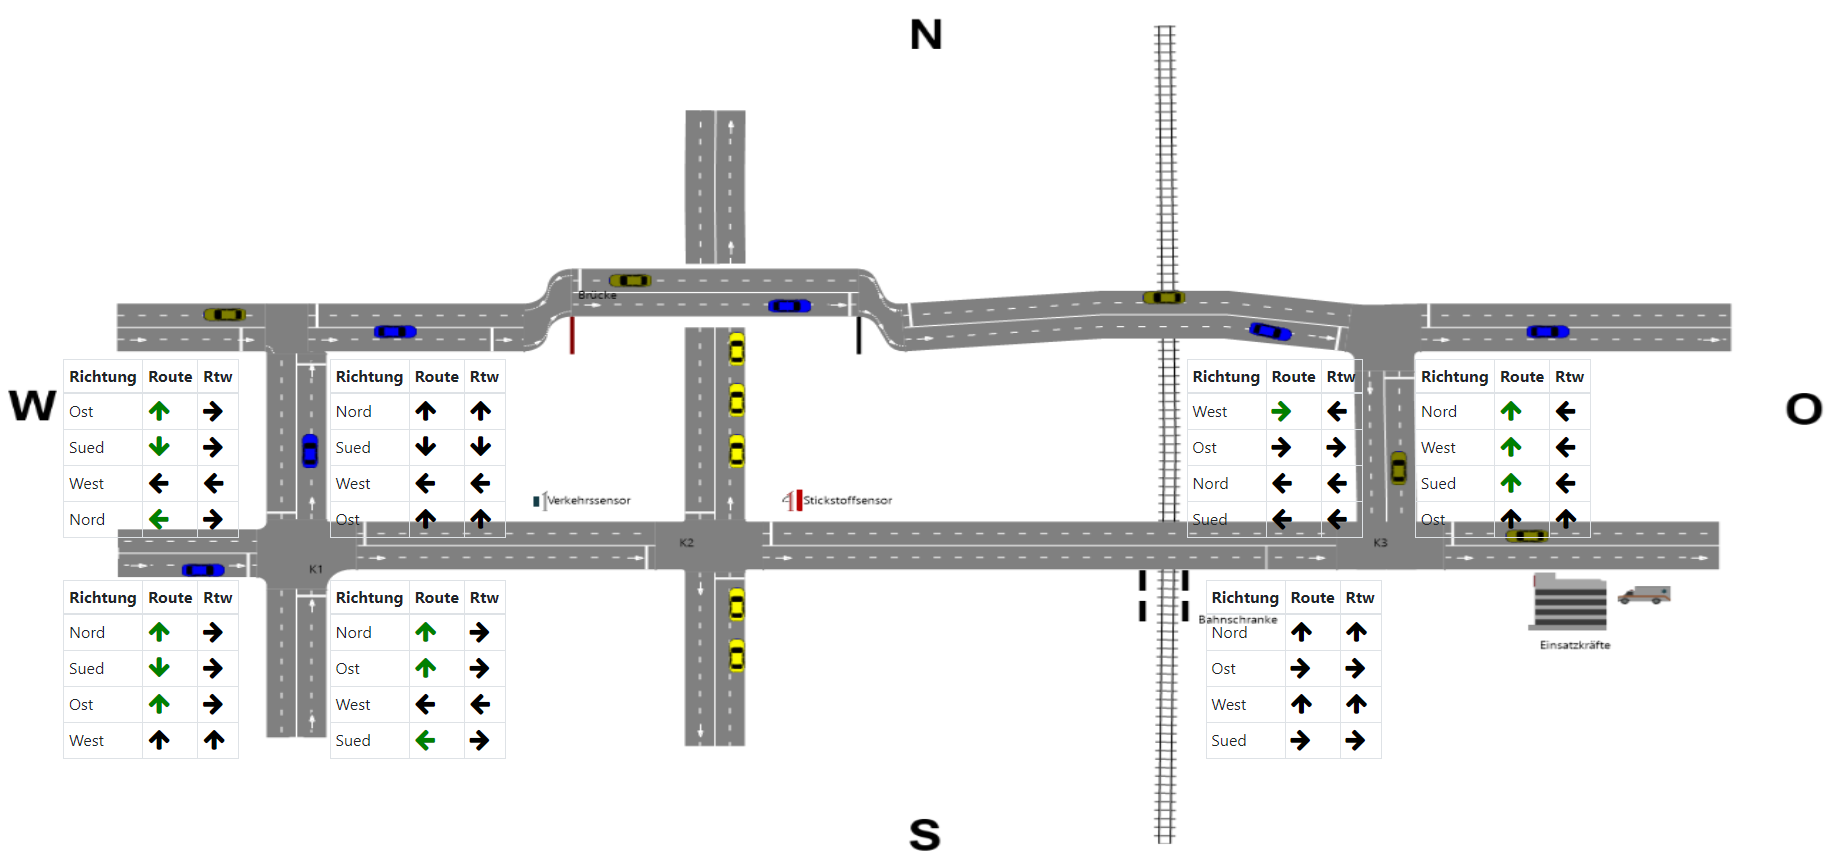
\includegraphics[width=\textwidth]{images/NitroOxigenStillHigh.png}
	\caption{Stickstoff-Alarm und Sperrung für den kompletten Verkehr außer Nord-Süd}
	\label{fig9}
\end{figure}


\subsection{Erhöhtes Verkehrsaufkommen}

Der Verkehrsstrom in der Fallstudie wird mit kontinuierlich erzeugten \textit{TrafficStartEvents} simuliert. Um festzustellen, ob  Vorkehrungen zur Entlastung der Straßen getroffen werden müssen, zählt das Statement

\begin{lstlisting}
select count(*) from TrafficStartEvent(direction = 'OtoW')#time(15 seconds) having (count(*) >5 and count(*) <= 6)
\end{lstlisting}

die Anzahl der Fahrzeug, die von Ost nach West oder vice versa fahren. Liegt die Anzahl der gemessenen Fahrzeuge in einem 15-Sekunden-Intervall zwischen fünf und sechs, wird der \textit{TrafficStartListener} ausgelöst. Die aktuelle Situation ist in Abb. \ref{fig10} veranschaulicht.

\begin{figure}[ht]
	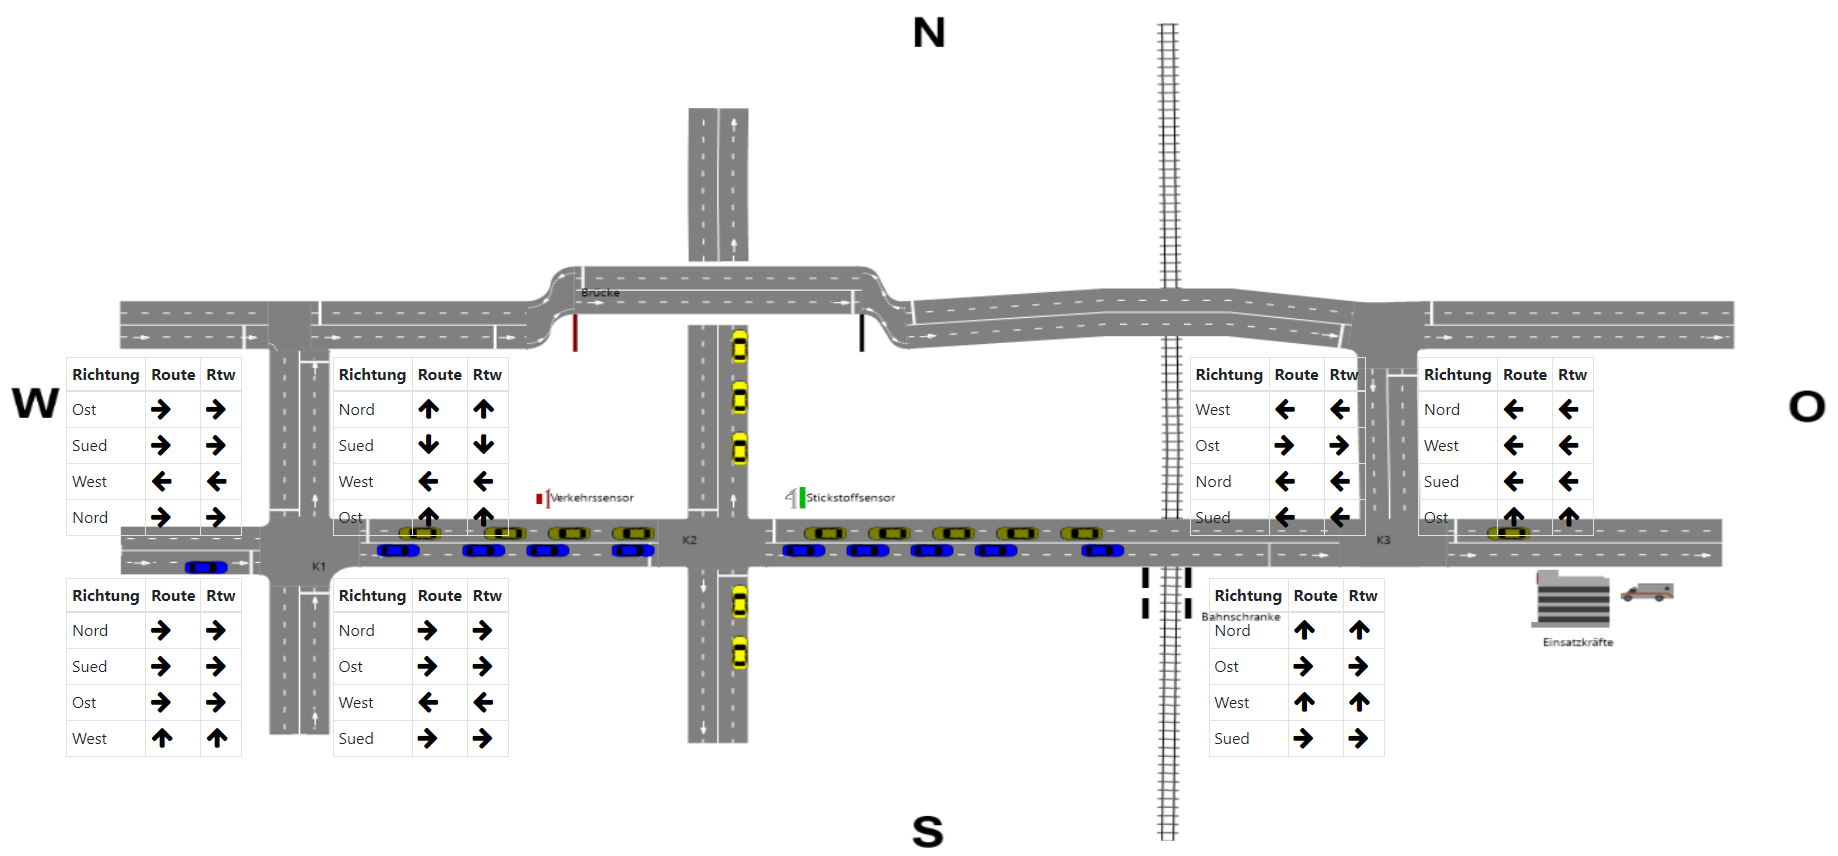
\includegraphics[width=\textwidth]{images/TrafficHigh.png}
	\caption{Hohe Verkehrsbelastung auf S1}
	\label{fig10}
\end{figure}


Ob mehr als sechs Fahrzeuge innerhalb von 15 Sekunden die Ost-West-Verbindung nutzen, wird durch das Statement
\begin{lstlisting}
select count(*) from TrafficStartEvent(direction = 'OtoW')#time(15 seconds) having count(*) >10
\end{lstlisting}
ermittelt. Daraufhin reagiert der \textit{TrafficTimeIntervalListener} und erzeugt eine Aufteilung des Verkehrs auf zwei Straßen. Wie in Abb. \ref{fig11} ersichtlich, nutzt der West-Ost-Verkehr nun die zweispurig befahrbare Straße S1. Der Ost-West-Verkehr wird auf die nun ebenfalls zweispurige Straße S2 umgeleitet. 

\begin{figure}[ht]
	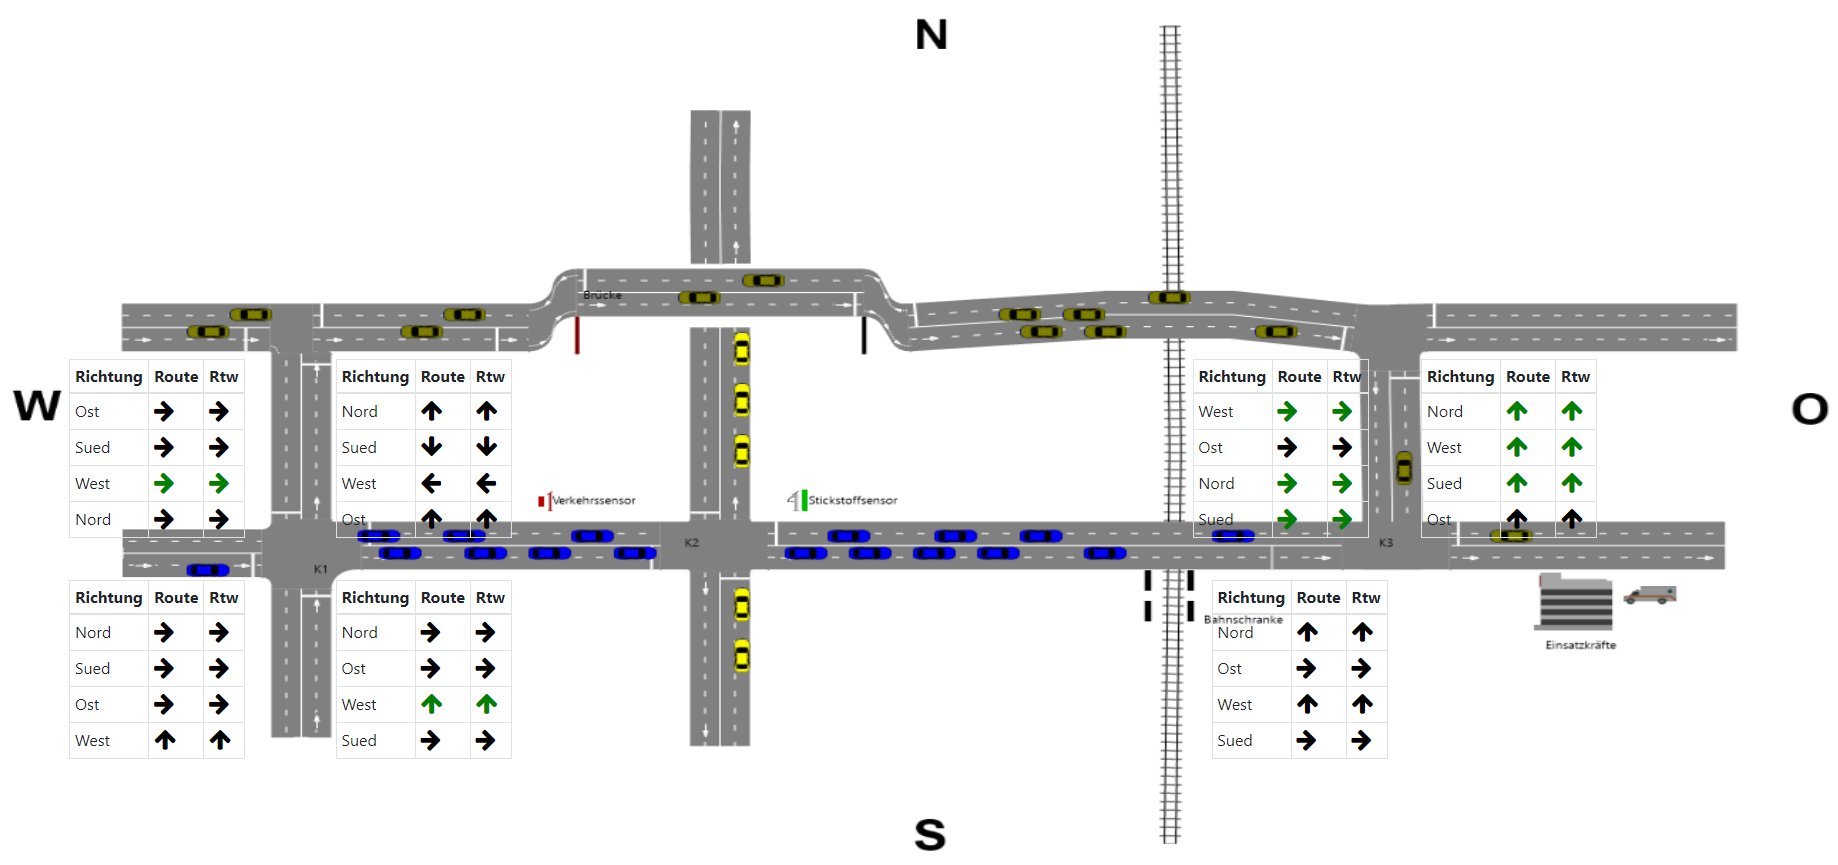
\includegraphics[width=\textwidth]{images/TrafficVeryHigh.png}
	\caption{Sehr hohe Verkehrsbelastung und Einrichtung einspuriger Fahrbahnen}
	\label{fig11}
\end{figure}

Das Statement 

\begin{lstlisting}
select count(*) from TrafficStartEvent(direction = 'OtoW')#time(15 seconds) having count(*) <= 3
\end{lstlisting}

erkennt das Ende der Verkehrsbelastung und startet den \textit{TrafficEndListener}, sobald sich die Anzahl der Fahrzeuge in beiden Richtungen auf drei oder weniger im 15 Sekunden-Intervall reduziert hat. Im Anschluss daran wird die Verkehrsführung in den Normalzustand zurück versetzt.\\

In diesem Kapitel wurde anhand eines fiktiven Verkehrsszenarios und real möglicher Ereignisse dargestellt, wie Event-Processing durch Esper realisiert werden kann. Dabei wurde deutlich, dass bei eintretenden Ereignissen immer auf eine Wechselwirkung mit anderen zeitnah eingetretenen Ereignissen geachtet werden muss. In diesem Zusammenhang wurden für das Fallbeispiel komplexe Ereignismuster definiert, erkannt und verarbeitet.

\clearpage
